\section{Preferences}


\subsection{Consumer Preferences}

\slide{Consumer Preferences}{
    So far, the discussion has focused on \emph{what the consumer can afford}.
    Now, the focus of the discussion will shift towards \emph{what the consumer wants}.

    In order to do this, consumer preferences need to be studied.

    The end goal of consumer theory and optimisation is to find how to derive maximum satisfaction,
    given the consumer's constraints.
    
    The topic of `Budget Constraint' focuses on the `consumer's constraints' part.
    Now, the discussion will move towards `how to derive maximum satisfaction'.
}


\slide{Consumer Preferences}{
    Suppose two goods exist in an economy; good 1 and good 2.

    We create two bundles \(X = (x_1, x_2)\) and \(Y = (y_1, y_2)\).

    \begin{itemize}
        \item We say the consumer \textbf{strictly prefers} bundle X to Y and write:
        \[(x_1, x_2) \succ (y_1, y_2)\]
        \item We say the consumer \textbf{weakly prefers} bundle X to Y and write:
        \[(x_1, x_2) \succeq (y_1, y_2)\]
        \item We say the consumer is \textbf{indifferent} between bundles X \& Y and write:
        \[(x_1, x_2) \sim (y_1, y_2)\]
    \end{itemize}
}


\subsection{Assumptions}

\slide{Assumptions (Axioms)}{
\begin{itemize}
    \item We assume that preferences are \textbf{complete}. This means that given any two
    bundles in the budget set, the consumer has a preference.
    \begin{itemize}
        \item For any two bundles either \((x_1, x_2) \succ (y_1, y_2)\) or \((x_1, x_2) \succeq (y_1, y_2)\)
        or both i.e. \((x_1, x_2) \sim (y_1, y_2)\).
    \end{itemize}

    \item We assume that preferences are \textbf{reflexive}. This means that any bundle is
    at least as good as itself.
    \begin{itemize}
        \item For any bundle \((x_1, x_2) \succeq (y_1, y_2)\).
    \end{itemize}

    \item We assume that preferences are \textbf{transitive}. This means that if bundle A is preferred
    to B, and B is preferred to C, then A is preferred to C.
    \begin{itemize}
        \item For any three bundles X, Y, and Z: \((x_1, x_2) \succeq (y_1, y_2)\) and \((y_1, y_2) \succeq (z_1, z_2)\)
        implies \((x_1, x_2) \succeq (z_1, z_2)\).
    \end{itemize}
\end{itemize}
}



\section{Indifference Curves}


\subsection{Indifference Curves}

\slide{Indifference Curves}{
    Suppose we pick an arbitrary bundle X (\(x_1, x_2\)).

    \dfn{Indifference curve is the set of all bundles that the consumer is indifferent between.
    In essence, the bundles that the consumer likes as much as \((x_1, x_2)\) make up the indifference curve.}

    An indifference curve is the representation of a consumer's preferences. Therefore, it
    must obey completeness, reflexivity, and transitivity.

    Then, all bundles that are weakly preferred to \((x_1, x_2)\) form the \\ \textbf{weakly preferred set}.
    We can then say that the indifference curve forms the boundary to the weakly preferred
    set of a bundle.
}


\slide{Indifference Curves Graphically}{
\begin{center}
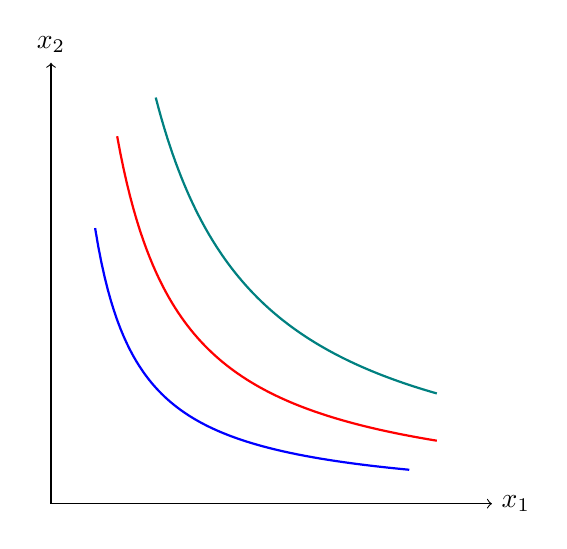
\begin{tikzpicture}[scale=0.7]
% Axes
\draw[->] (0,0) -- (8,0) node[right] {$x_1$};
\draw[->] (0,0) -- (0,8) node[above] {$x_2$};

% Indifference curve (example: x1 * x2 = 4  =>  x2 = 4/x1)
\draw[blue, thick, domain=0.8:6.5, samples=100]
    plot (\x, {4/\x});

\draw[red, thick, domain=1.2:7, samples=100]
    plot (\x, {8/\x});

\draw[teal, thick, domain=1.9:7, samples=100]
    plot (\x, {14/\x});
\end{tikzpicture}
\end{center}
}


\slide{Weakly Preferred Set}{
\begin{center}
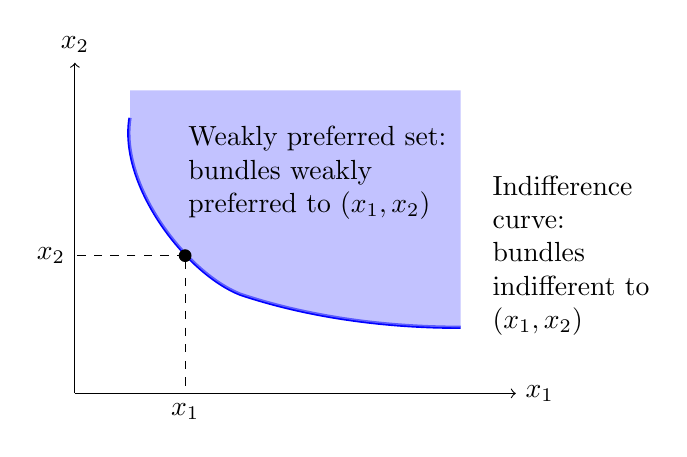
\begin{tikzpicture}[scale=0.7]

% Axes
\draw[->] (0,0) -- (8,0) node[right] {$x_1$};
\draw[->] (0,0) -- (0,6) node[above] {$x_2$};

% Indifference curve
\draw[very thick, blue]
    (1,5) .. controls (0.8,3.8) and (2,2.2) ..
    (3,1.8) .. controls (4.5,1.3) and (6,1.2) ..
    (7,1.2);

% Shaded weakly preferred set (area above curve)
\fill[blue!40, opacity=0.6]
    (1,5) 
    .. controls (0.8,3.8) and (2,2.2) ..
    (3,1.8) 
    .. controls (4.5,1.3) and (6,1.2) ..
    (7,1.2)
    -- (7,5.5)
    -- (1,5.5)
    -- cycle;

% Point (x1, x2)
\filldraw[black] (2,2.5) circle (3pt);

% Dashed projection lines
\draw[dashed] (2,2.4) -- (2,0);
\draw[dashed] (2,2.5) -- (0,2.5);

% Axis point labels
\node[below] at (2,0) {$x_1$};
\node[left] at (0,2.5) {$x_2$};

% Text annotations
\node[align=left] at (4.4,4)
{Weakly preferred set:\\
bundles weakly\\
preferred to $(x_1,x_2)$};

\node[align=left] at (9,2.5)
{Indifference\\
curve:\\
bundles\\
indifferent to\\
$(x_1,x_2)$};

\end{tikzpicture}
\end{center}
}


\slide{Indifference Curves Never Cross}{
    We require that indifference curves never cross. Why?

    \begin{center}
    \begin{tikzpicture}[scale=0.8]
    % Axes
    \draw[->] (0,0) -- (6,0) node[right] {$x_1$};
    \draw[->] (0,0) -- (0,6) node[above] {$x_2$};

    % First indifference curve: x1
    \draw[red, thick, domain=0.8:3.5, samples=100]
        plot (\x, {4/\x - 1});
        \filldraw[black] (1.05,2.8) circle (2pt);
        \node[above right] at (1.05,2.9) {$B$};

    % Second indifference curve: x2
    \draw[blue, thick, domain=0.5:5]
        plot (\x, {2/\x});
        \filldraw[black] (0.7,2.9) circle (2pt);
        \node[above right] at (-0.15,2.8) {$A$};

    \filldraw[black] (2,1) circle (2pt);
    \node[above right] at (2,1) {$C$};
    \end{tikzpicture}
    \end{center}
}

\slide{Indifference Curves Never Cross}{
    In the previous diagram, bundle B is in the weakly preferred set of bundle A. Therefore,
    the consumer (weakly) prefers bundle B to A.

    Furthermore, the consumer is indifferent between bundle A and C because they lie
    on the same indifference curve.

    However, the consumer is also indifferent between bundle C and B as they lie
    on the same indifference curve. By transitivity, if \(A \sim C\) and \(C \sim B\),
    it must be true that \(A \sim B\).

    There is a contradiction. This is why two indifference curves must not intersect.
}


\subsection{Perfect Substitutes}


\slide{Perfect Substitutes}{
    Two goods are perfect substitutes if the consumer is willing to substitute
    one good for the other at a \emph{constant rate} (two-for-one or one-for-one).

    Suppose that there is a choice between coca-cola and pepsi, and the consumer
    involved does not care about which drink they get at all.

    Pick a consumption bundle, say (10,10). Then for this consumer, any other
    consumption bundle that has 20 drinks in it is just as good as (10,10).
    
    Mathematically, any consumption bundle \((x_1, x_2)\) such that \(x_1 + x_2 = 20\)
    will be on the consumer's indifference curve. Thus, the indifference curves for this
    consumer are all parallel straight lines with a slope of -1.
}


\slide{Perfect Substitutes Graphically}{
\begin{center}
\begin{tikzpicture}[scale=0.9]

% Axes
\draw[->] (0,0) -- (7,0) node[right] {$x_1$ (Coca-Cola)};
\draw[->] (0,0) -- (0,7) node[above] {$x_2$ (Pepsi)};

% Indifference curves: x2 = k - x1
\draw[thick, blue] (0,6) -- (6,0);
\draw[thick, blue] (0,5) -- (5,0);
\draw[thick, blue] (0,4) -- (4,0);

% Labels for curves
\node[right] at (-1.4,6) {$u=6$};
\node[right] at (-1.4,5) {$u=5$};
\node[right] at (-1.4,4) {$u=4$};

\end{tikzpicture}
\end{center}
}


\subsection{Perfect Complements}


\slide{Perfect Complements}{
    Perfect complements are goods that are always consumed together in
    fixed proportions. A nice example is that of right shoes and left shoes.
    Having only one out of a pair of shoes doesn't do the consumer a bit of good.

    Suppose we pick the consumption bundle (10,10). Now add 1 more right shoe, so
    we have (11,10). This leaves the consumer indifferent to
    the original position: the extra shoe doesn't do him any good.

    The same thing happens if we add one more left shoe: the consumer is also indifferent
    between (10,11) and (10,10).

    Thus the indifference curves are L-shaped, with the optimal number of shoes being at the
    vertex of the L where the number of left shoes equals the number of right shoes.
}


\slide{Perfect Complements Graphically}{
\begin{center}
\begin{tikzpicture}[scale=0.9]

% Axes
\draw[->] (0,0) -- (7,0) node[right] {$x_1$ (Right Shoe)};
\draw[->] (0,0) -- (0,7) node[above] {$x_2$ (Left Shoe)};

% Indifference curve u = 2
\draw[thick, blue] (2,7) -- (2,2) -- (7,2);

% Indifference curve u = 3
\draw[thick, blue] (3,7) -- (3,3) -- (7,3);

% Indifference curve u = 4
\draw[thick, blue] (4,7) -- (4,4) -- (7,4);

% Labels
\node[left] at (3.25,2.4) {$u=2$};
\node[left] at (4.25,3.4) {$u=3$};
\node[left] at (5.25,4.4) {$u=4$};

\end{tikzpicture}
\end{center}
}


\subsection{Bads, Neutral Goods, and Satiation}


\slide{Bads}{
    A bad is a commodity that the consumer doesn't like (as opposed to a good).
    
    For example, suppose that the commodities in question are now pepperoni and anchovies —
    and the consumer loves pepperoni but dislikes anchovies.

    Let us suppose there is some possible tradeoff between pepperoni and anchovies. That is,
    there would be some amount of pepperoni on a pizza that would compensate the
    consumer for having to consume a given amount of anchovies.

    Pick a bundle \((x1,x2)\) consisting of some pepperoni and some anchovies.
    If we give the consumer more anchovies, what do we have to do with the
    pepperoni to keep him on the same indifference curve?

    Clearly, we have
    to give him some extra pepperoni to compensate him for having to put up
    with the anchovies. Thus this consumer must have indifference curves that
    slope up and to the right.
}


\slide{Bads Graphically}{
\begin{center}
\begin{tikzpicture}[scale=0.9]

% Axes
\draw[->] (0,0) -- (7,0) node[right] {$x_1$ (\text{Pepperoni})};
\draw[->] (0,0) -- (0,7) node[above] {$x_2$ (\text{Anchovies})};

% Indifference curves: x2 = x1 - k
\draw[thick, blue] (1,0) -- (7,6);
\draw[thick, blue] (2,0) -- (7,5);
\draw[thick, blue] (3,0) -- (7,4);

% Labels
\node[right] at (7,6) {$u=1$};
\node[right] at (7,5) {$u=2$};
\node[right] at (7,4) {$u=3$};

\end{tikzpicture}
\end{center}
}


\slide{Neutral Goods}{
    A good is a neutral good if the consumer doesn't care about it one way
    or the other. What if a consumer is just neutral about anchovies?

    He only cares about the amount of pepperoni he has and doesn't care at
    all about how many anchovies he has. The more pepperoni the better, but
    adding more anchovies doesn't affect him one way or the other.
}


\slide{Neutral Goods Graphically}{
\begin{center}
\begin{tikzpicture}[scale=0.9]

% Axes
\draw[->] (0,0) -- (7,0) node[right] {$x_1$ (Pepperoni)};
\draw[->] (0,0) -- (0,7) node[above] {$x_2$ (Anchovies)};

% Indifference curves: x1 = k
\draw[thick, blue] (2,0) -- (2,6.5);
\draw[thick, blue] (3.5,0) -- (3.5,6.5);
\draw[thick, blue] (5,0) -- (5,6.5);

% Labels
\node[below] at (2,0) {$u=2$};
\node[below] at (3.5,0) {$u=3.5$};
\node[below] at (5,0) {$u=5$};

\end{tikzpicture}
\end{center}
}


\slide{Satiation}{
    We sometimes want to consider a situation involving satiation, where
    there is some overall best bundle for the consumer, and the “closer” he is
    to that best bundle, the better off he is in terms of his own preferences.

    In this case we say that \((x_1,x_2)\) is a satiation point, or a bliss point.

    Suppose, for example, that the two goods are chocolate cake and ice
    cream. There might well be some optimal amount of chocolate cake and
    ice cream that you would want to eat per week. Any less than that amount
    would make you worse off, but any more than that amount would also make
    you worse off.
}


\slide{Satiation}{
\begin{center}
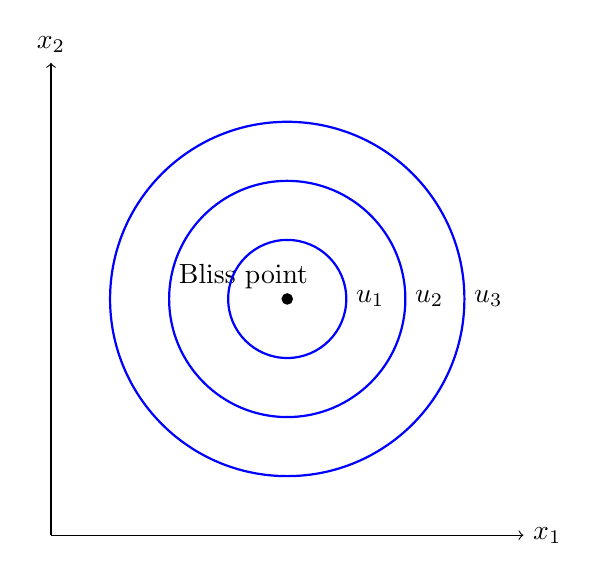
\begin{tikzpicture}[scale=0.75]

% Axes
\draw[->] (0,0) -- (8,0) node[right] {$x_1$};
\draw[->] (0,0) -- (0,8) node[above] {$x_2$};

% Bliss point
\filldraw[black] (4,4) circle (2.5pt);
\node[above right] at (2,4) {Bliss point};

% Indifference curves (concentric circles)
\draw[thick, blue] (4,4) circle (1);
\draw[thick, blue] (4,4) circle (2);
\draw[thick, blue] (4,4) circle (3);

% Labels
\node[right] at (5,4) {$u_1$};
\node[right] at (6,4) {$u_2$};
\node[right] at (7,4) {$u_3$};

\end{tikzpicture}
\end{center}
}



\section{Well-Behaved Preferences}


\subsection{General Preferences}

\slide{General Preferences}{
    We have seen that many kinds of preferences, reasonable or unreasonable, can be described by
    indifference curves.
    
    However, if we want to describe preferences in general, it will
    be convenient to focus on a few general shapes of indifference curves.

    We will now describe some more general assumptions that we will
    typically make about preferences and the implications of these assumptions
    for the shapes of the associated indifference curves.

    These assumptions are not the only possible ones; in some situations you might want to use
    different assumptions. But we will take them as the defining features for
    \emph{well-behaved indifference curves}.
}


\subsection{Monotonicity}

\slide{Monotonicity}{
    \dfn{Monotonicity is the assumption that more of a good is better than less.
    More precisely, if \((x_1,x_2)\) is a bundle of goods and \((y_1,y_2)\) is a bundle of goods
    with at least as much of both goods and more of one, then \((y_1,y_2) \succ (x_1,x_2)\).}

    As suggested in the discussion of satiation, more is better probably only
    hold up to a certain point. Thus the assumption of monotonicity is saying that we are going
    to examine situations before that point is reached — before any satiation sets in — while more still is better.

    What does monotonicity imply about the shape of indifference curves?
    It implies that they have a negative slope.
}


\slide{Monotonicity Graphically}{
    \begin{center}
        \includegraphics[scale=0.4]{MONOTONE1}
    \end{center}
}



\subsection{Convexity}

\slide{Convexity}{
    \dfn{Preferences are said to be convex if, for any two bundles that a consumer finds equally desirable,
    any weighted average (or combination) of these bundles is at least as desirable as either of the original bundles.
    In essence, we are going to assume that averages are preferred to extremes.}

    If we take two bundles of goods \((x_1,x_2)\) and \((y_1,y_2)\) on the same
    indifference curve and take a weighted average of the two bundles such as:
    \[\left( \frac{1}{2}x_1 + \frac{1}{2}y_1 , \frac{1}{2}x_2 + \frac{1}{2}y_2 \right)\]
    then the average bundle will be at least as good as or strictly preferred
    to each of the two extreme bundles.
}


\slide{Convexity}{
    To be more precise, given two bundles such that \((x_1, x_2) \sim (y_1, y_2)\).
    We're going to assume that for any weight \(t\) between 0 and 1:
    \[\left( tx_1 + [1-t]y_1, tx_2 + [1-t]y_2 \right) \succeq (x_1, x_2)\]

    What does this assumption about preferences mean geometrically?
    It means that the \emph{weakly preferred set} of the bundle \((x1,x2)\) is a \textbf{convex set}.

    \dfn{A convex set has the property that if you take any two points in the set and draw the
    line segment connecting those two points, that line segment lies entirely in the set.}
}


\slide{Convexity Graphically}{
    \begin{center}
        \includegraphics[scale=0.4]{CONVEX1}
    \end{center}
}